\section{Variables}
\subsection{Independent Variables and Dependent Variables}
The independent variable for this experiment is the temperature of the NTC Thermistor, which is measured by a Vernier Temperature Probe with a precision of $\pm 0.1^\circ C$. The dependent variable for my experiment is the electrical resistance of the NTC Thermistor, which is measured using a Multimeter configured as an Ohmmeter with a precision of $\pm 0.01 \; k\Omega$.

Since all data is being collected after running all trials, the high precision of video analysis can be utilized, which greatly increases both the accuracy and precision of the resistance and temperature data. More details about the specific measurement processes are described in the Section \ref{section:procedure} \nameref{section:procedure}.

\subsection{Control Variables}
I ensured that all other variables were controlled to get accurate results about the relationship between the resistance and temperature. For example, throughout the trials, the circuit remained untouched so that no variations would occur due to the connections. Furthermore, the same amount of water ($150 \; mL$) at roughly the same initial temperature ($<20^\circ C$) was used for every trial with the same heating source to ensure that the controlled temperature increased at the same rate throughout the trials. Finally, the beaker, temperature probe, and thermistor were always cooled down to room temperature before proceeding to do a new trial. Through all measures, a more accurate relationship between my independent and dependent variables can be assessed.

\section{Methodology}
\subsection{Materials}
\begin{itemize}[noitemsep]
    \item NTC Thermistor (E305314; HXT-600; Max Operating Temperature: $105^\circ C$)
    \item Vernier Temperature Probe, $\pm 0.1^\circ C$
    \item GoLink (for connecting to Logger Pro)
    \item Logger Pro Software on Laptop (for dynamic temperature logging)
    \item Multimeter (as use as Ohmmeter), $\pm 0.01 \; k\Omega$ 
    \item Heat Source (Gas Stovetop used in this experiment, though Bunsen Burner or Heating Plate could be used)
    \item Phone and Tripod Stand (to record experiment)
    \item $400 \; mL$ Glass Beaker
    \item Beaker Tongs and Wire Gauze (to move hot beaker and evenly heat up and cool down beakers respectively)
    \item $150 \; mL$ of Water initially at $<20^\circ C$ (medium to heat up thermistor)
\end{itemize}

\subsection{Experimental Setup}
\begin{figure}[ht]
    \centering
    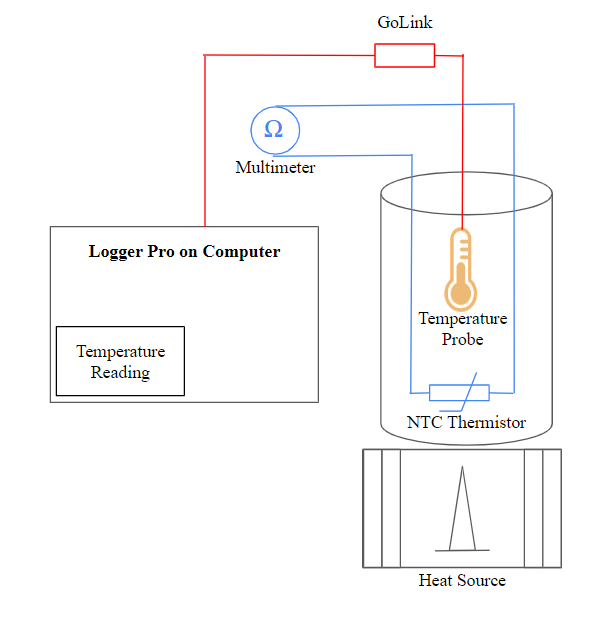
\includegraphics[width=\textwidth,height=100mm,keepaspectratio]{images/IA_Schematic.png}
    \caption{Schematic for Physics IA Experiment Setup}
    \label{fig:schematic}
\end{figure}


\begin{figure}[ht]
    \centering
    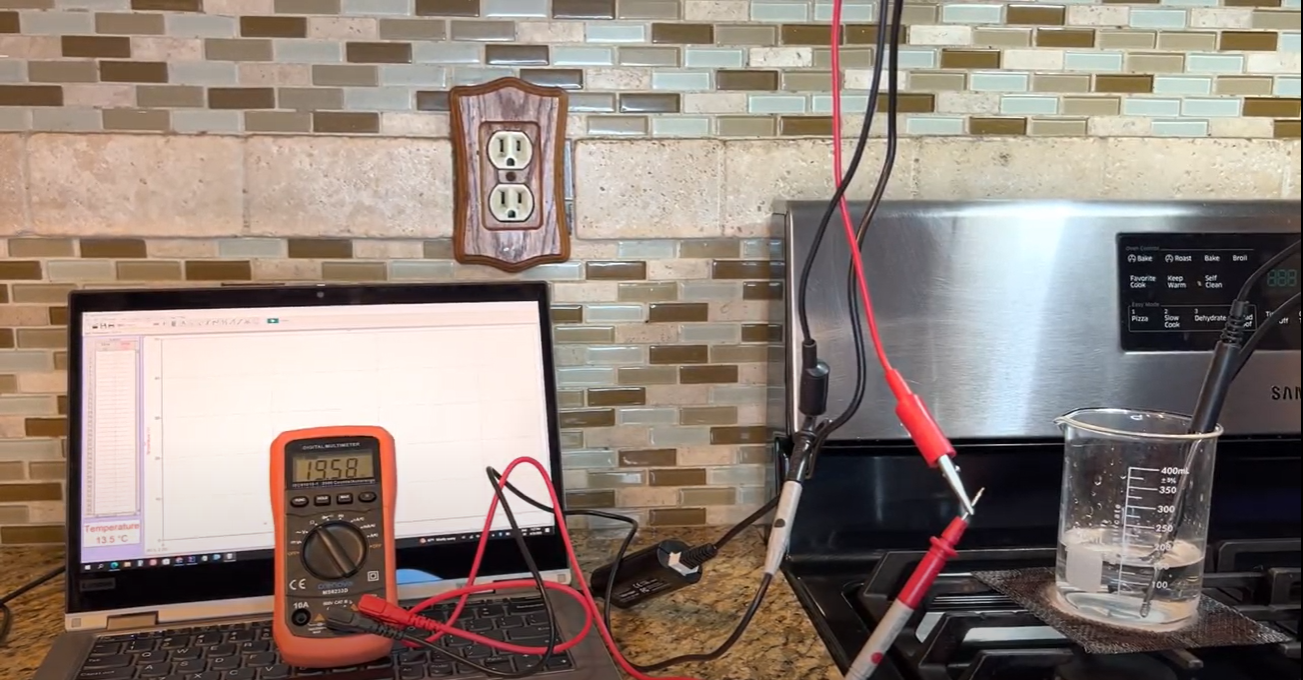
\includegraphics[width=120mm,height=\textheight,keepaspectratio]{images/setup.png}
    \caption{Example Image of Phone Footage at Start of Experiment}
    \label{fig:footage}
\end{figure}

\section{Procedure}
\label{section:procedure}
\begin{enumerate}[noitemsep]
    \item Put Multimeter in Ohmmeter mode and attach each of the leads to the thermistor leads. Plug Vernier Temperature Probe into the laptop via the GoLink. Open up Logger Pro software to get live temperature reading. Place Wire Gauze on Gas Stovetop. Setup the Tripod Stand with Phone such that the Multimeter and Temperature Probe readings are clearly visible.
    \item Now, for each of the 5 trials:
    \begin{enumerate}[noitemsep]
        \item Fill the Glass Beaker with $150 \; mL$ of water, which is initially below $20^\circ C$, and place it on the Wire Gauze. Put the Temperature Probe and the NTC Thermistor near the center of the beaker.
        \item Start recording the trial using the phone-tripod setup. Put the heat at the lowest setting so that the temperature rises slowly and evenly.
        \item once the water starts boiling at $~100^\circ C$, end the recording and turn off the heating from the stove. Remove the Temperature Probe and NTC Thermistor from the Beaker. Use the Beaker Tongs to carry the hot beaker and dump out the boiling water. Leave the Glass Beaker on the Wire Gauze to cool back down to room temperature.
    \end{enumerate}
    \item Using all the footage collected in the previous step, the 16 levels of resistance and temperature data points must be collected. For each video:
    \begin{enumerate}[noitemsep]
        \item Slowly scroll through the video till you get to exactly $20.0^\circ C$. Record the resistance reading at this temperature in a table.
        \item Repeat this process in $5^\circ C$ increments until $95^\circ C$ is reached. 
    \end{enumerate}
\end{enumerate}

\section{Safety and Ethics}
Throughout this investigation, all safety and ethical concerns were recognized and thoroughly addressed. The main hazard in this lab is the heating source. Thus, multiple solutions were implemented to mitigate risks. First, the experiment was approved and performed under teacher supervision. Second, proper experiment apparatus such as wire gauze and beaker tongs were used. Finally, the glass beaker was cooled slowly to ensure that it would not shatter upon a rapid temperature change. All these measures greatly improved safety, leading to no injuries during the course of the experiment.